\documentclass[times, utf8, zavrsni]{fer}
\usepackage{booktabs}
\usepackage{graphicx}
\usepackage{amsmath}
\usepackage{physics}
\usepackage{ctable}
\usepackage{algorithm}
\usepackage{algorithmic}

\graphicspath{ {./images/} }

\begin{document}

% TODO: Navedite broj rada.
\thesisnumber{000}
\title{Genetski algoritmi inspirirani kvantnom mehanikom}
\author{Juraj Fulir}
\maketitle

% Ispis stranice s napomenom o umetanju izvornika rada. Uklonite naredbu \izvornik ako želite izbaciti tu stranicu.
\izvornik

% Dodavanje zahvale ili prazne stranice. Ako ne želite dodati zahvalu, naredbu ostavite radi prazne stranice.
\zahvala{
  
Zahvaljujem svome mentoru prof. dr. sc. Domagoju Jakoboviću na danoj mogućnosti vlastitog odabira teme završnog rada te iznimnom interesu za istu. \\
Zahvaljujem svojoj obitelji na svoj podršci i strpljenju pogotovo tijekom kasnih noćnih sati. \\
Za kraj zahvaljujem Karlu Kneževiću, mag. ing., na kolegijalnoj pomoći.
}

\tableofcontents

\chapter{Uvod}
Sve do početka 19. stoljeća fizičari su imali deterministički pogled na svijet. Razvijanjem tehnologije koja je omogućavala promatranje sve manjih čestica primjećuju se čudni fenomeni koje dotadašnja fizika nije mogla opisati. Iz potrebe za objašnjavanjem tih neobićnih pojava razvijene su podjednako neobićne teorije koje, iako su matematički dokazane, nisu olako prihvaćene na znanstvenoj sceni. Jedna takva teorija je pretpostavka diskretne prirode stvarnosti. Iz nje je nastalo jedno čitavo područje fizike zvano '\it kvantna mehanika\rm '. Iako su puno ranije postojala slična razmišljanja o diskretnim i točkastim česticama (Galilei, Bošković), do 19. stoljeća nije postojala ni tehnologija kojom bi se tvrdnje dokazale ni matematika kojom bi se tvrdnje opisale.

\paragraph{}
Početkom 19. stoljeća, Max Planck objavljuje \it Plankov zakon zračenja\rm\ kojim rješava dugogodišnji problem zračenja crnog tijela, popularno nazvan "\it ultraljubičasta katastrofa\rm". Definira povezanost izračene energije s valnom duljinom izračene svjetlosti, ali još bitnije definira diskretizirano zračenje u paketićima energije koje naziva 'količina', latinski 'kvantum'. Njegovim otkrićem kreće revolucija u fizici od kojih ću spomenuti samo nekoliko: otkriće fotoelektričnog efekta (Einstein), ispravljanje (redefiniranje) modela atoma (Rutherford, Bohr), otkriće dvojne prirode čestica (De Broglie), opisivanje valne prirode elektronske ljuske atoma (Heisenberg, Schr\"odinger, Born).

\paragraph{}
Danas je kvantni pogled na svijet vrlo uvriježen u krugu fizičara, ali i šire no još nije u potpunosti shvaćen. Unatoč tome korištenjem fenomena proizišlih iz kvantne fizike stvorili smo razne uređaje i alate koji su danas u širokoj primjeni. Neki takvi uređaji su: tunel dioda, laser, magnetska rezonancija i drugi.

\paragraph{}
Ukratko, kvantna mehanika je relativno mlada grana fizike, ali je uvelike utjecala na naš razvoj tehnologije, znanosti i shvaćanja svijeta u kojem živimo.

\section{Kvantni algoritmi i kvantna računala}

\paragraph{}
\it No Clone Theorem\rm\ potvrđuje da nije moguće stvoriti kopiju postojećeg qbita odnosno nije moguće prenijeti kvantno stanje jednog qbita na drugi.

\paragraph{}
Primjenom qBita, teoretski je moguće ostvariti značajna ubrzanja nekih NP problema kvantnim algoritama (Shor-ov algoritam faktorizacije cijelih brojeva, Grover-ov algoritam pretrage nesortiranih polja, ...).
Jedan primjer primjene qbita je kvantni registar kao spremnik podataka, kojim se opisuje značaj superpozicije:
\begin{quote}
Pomoću 1 klasičnog registra velićine n bitova moguće je pohraniti 1 od mogućih $2^n$ vrijednosti.

Pomoću 1 kvantnog registra velićine n qBita moguće je pohraniti $2^n$ od mogućih $2^n$ vrijednosti, odnosno sve vrijednosti od jednom.
\end{quote}

\section{Trenutno stanje u svijetu}
Postoje dvije tvrtke koje danas izrađuju i razvijaju kvantna računala.

\subsection{D-Wave}
Tvrtka D-Wave razvija i proizvodi kompaktne zatvorene sustave kvantnih računala. Trenutno najnoviji model kvantnog računala tvrtke D-Wave je 2000Q, podržava 2000 qbita i temelji se na adijabatskom kvantnom računanju. Taj princip vrlo je sličan principu kvantnog kaljenja. Radi se o topološkom pretraživanju prostora stanja za koji se mogu modelirati neki problemi.
Ta su računala nedostupna široj javnosti isključivo radi cijene (15 milijuna američkih dolara 05.2017.) no neke su ih tvrke ipak nabavile (Google, NASA, USRA, Volkswagen Group i ostali).

\subsection{IBM}
Razvivši svoje kvantno računalo, IBM nudi udaljeni pristup svojim kvantnim računalima. Javni paket uključuje pristup web aplikaciji za dizajniranje kvantnih krugova do 5 qbita te mogućnost izvršavanja eksperimenta na simulatoru ili stvarnom kvantnom procesoru. Pristup stvarnom kvantnom procesoru naplaćuje se 'virtualnim kreditom' koji se dobije registracijom na sustav i vremenski obnavlja. Svako izvršavanje se naplaćuje ovisno o zadanom broju ponovljanja eksperimenta. Početkom 2017. godine omogućen je pristup računalu s čak 20 qbita preko web aplikacije.

\chapter{Kvantni bit (qbit)}
Kvantni bit je najmanja jedinica podatka u kvantnim računalima. Fizički je to zapravo sićušna čestica sa svojstvom superpozicije, jedne od temeljnih fizikalnih pojava u "kvantnom svijetu" čiju ćemo primjenu objasniti u nastavku.

\section{Princip rada}
\paragraph{}
Klasični bit pronalazimo u jednom od dva klasična stanja. Jednom postavljeno stanje se pamti i uvijek ga u njemu možemo pronaći. Njima gradimo binarni brojevni sustav pomoću kojeg zapisujemo podatke na računalu.

\paragraph{}
Kvantni bit ne pamti jedno klasično stanje već se on istovremeno nalazi u više različitih klasičnih stanja. To se svojstvo naziva superpozicija. Fizički gledano kvantni bit je čestica kojoj je pridružen kvantizirani spin. Spin je kvantizirana inačica kutne količine gibanja rotirajućeg tijela.

\paragraph{}
Kvantno stanje jednog qubita opisano je vektorom njegovog spina. Kvantno stanje opisuje vjerojatnost pronalaženja qbita u svakom od klasičnih stanja. Konkretno stanje dobivamo mjerenjem qbita kojim se uništava njegovo svojstvo superpozicije te dobivamo česticu u jednom stanju koju možemo koristiti poput klasičnog bita.

\begin{center}
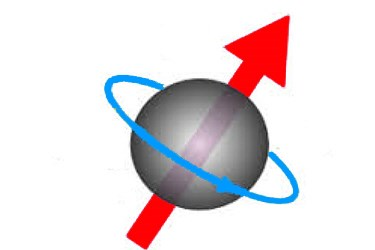
\includegraphics[width=55mm, height=40mm]{spin}
\captionof{figure}{Vjerojatnost pronalaženja qbita u određenom stanju opisana je njegovim kvantnim stanjem (spinom).}
\end{center}

\paragraph{}
Sustavi s kvantnim bitovima mogu biti definirani za proizvoljan brojevni sustav, no kako su današnja računala bazirana na binarnom brojevnom sustavu zanima nas definicija qbita s 2 stanja.

\subsection{Blochova shema}
\paragraph{}
Stanje qbita prikazujemo Blochovom shemom. Jedno kvantno stanje prikazujemo kao vektor iz središta sfere na njezinu površinu. Stanja u kojima možemo pronaći qbit prikazujemo polovima sfere koje definiramo sjecištima sfere i z-osi.

\begin{center}
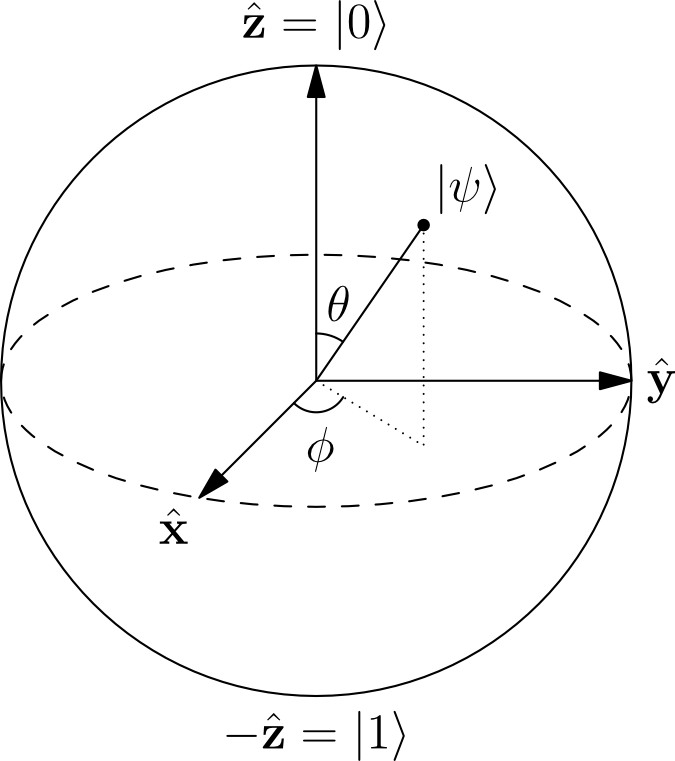
\includegraphics[width=60mm, height=65mm]{bloch}
\captionof{figure}{Blochova sfera}
\end{center}

\paragraph{}
Na slici vidimo jedno kvantno stanje opisano vektorom. Matematički ga možemo opisati kao linearnu kombinaciju dvaju klasičnih stanja:

\begin{align}
\ket{\psi} &= \alpha\ket{0} + \beta\ket{1} \label{eq:psi_orig}
\end{align}

\paragraph{}
Iz Blochove sfere popunjavamo konstante iz \eqref{eq:psi_orig}:

\begin{align}
\ket{\psi} &= \cos(\frac{\theta}{2})\ket{0} + e^{i\phi}\sin(\frac{\theta}{2})\ket{1} \nonumber \\
&= \cos(\frac{\theta}{2})\ket{0} + (cos(\phi)+i\sin(\phi))\sin(\frac{\theta}{2})\ket{1} \label{eq:psi_orig_full}
\end{align}

\paragraph{}
Vrijednosti $\alpha$ i $\beta$ su normirane:

\begin{equation} \label{eq:prob_norm}
|\alpha|^2 + |\beta|^2 = 1
\end{equation}

\paragraph{}
Vrijednosti $\alpha$ i $\beta$ predstavljaju vjerojatnosne amplitude pronalaženja qbita u stanju $\ket{0}$ i $\ket{1}$ respektivno.
Iz vjerojatnosnih amplituda računamo vjerojatnosti pronalaženja qbita u svakom od stanja:

\begin{equation} \label{eq:prob}
\begin{split}
\Pr{\ket{0}} = |\alpha|^2 = \cos^2{\frac{\theta}{2}} \\ 
\Pr{\ket{1}} = |\beta|^2 = \sin^2{\frac{\theta}{2}}
\end{split}
\end{equation}

\paragraph{}
Kvantno stanje kraće možemo napisati u obliku vektora:

\begin{equation} \nonumber
\ket{\psi} =
\begin{pmatrix}
\alpha \\ \beta
\end{pmatrix}
\end{equation}

\subsection{Aproksimacija kvantnog stanja}
\paragraph{}
Kvantno stanje prikazano na Blochovoj sferi opisano je u 3 dimenzije. Kako su operacije nad 3 dimenzije računski zahtjevne želimo pojednostaviti model kvantnog stanja. 
U simulaciji qbita jedino su nam važne vjerojatnosti pronalaženja qbita u određenom stanju. 
Ako pogledamo kvantno stanje opisano formulom \eqref{eq:psi_orig_full} vidimo da $\alpha$ ovisi samo o kutu $\theta$. Kombinacijom formula \eqref{eq:psi_orig_full} i \eqref{eq:prob_norm} zaključujemo kako $\beta$ ovisi isključivo o $\alpha$:

\begin{align*}
|\alpha|^2 + |\beta|^2 &= 1 \\
|\beta|^2 &= 1 - |\alpha|^2 \\
&= 1 - \cos^2(\frac{\theta}{2}) \\
&= \sin^2(\frac{\theta}{2})
\end{align*}

\paragraph{}
Zaključujemo da je kut $\phi$ suvišan. To možemo vidjeti i na samoj Blochovoj sferi.
Za fiksni kut $\theta$ mijenjanjem kuta $\phi$ rotiramo vektor oko z-osi i ne približavamo se niti jednom polu sfere.

\paragraph{}
Dobivamo sljedeću reprezentaciju kvantnog stanja qbita:

%%%%%%%%%%%%%%%%%
SLIKA 2D

\begin{equation}
\ket{\psi} = \cos(\frac{\theta}{2})\ket{0} + \sin(\frac{\theta}{2})\ket{1}
\end{equation}

\section{Kvantni registar}
Kvantni registar, poput klasičnog registra, pohranjuje niz qbita te omogućuje ne-destruktivno čitanje i zapisivanje istih.
\begin{align*}
\begin{bmatrix}
q_1 & q_2 & q_3 & \cdots & q_i & \cdots & q_n
\end{bmatrix}
\end{align*}

Simulacija kvantnog registra je klasični registar koji pohranjuje vjerojatnosti qbita:
\begin{align*}
\begin{bmatrix}
\alpha_1 & \alpha_2 & \alpha_3 & \cdots & \alpha_i & \cdots & \alpha_n \\
\beta_1 & \beta_2 & \beta_3 & \cdots & \beta_i & \cdots & \beta_n
\end{bmatrix}
\end{align*}

Nadalje možemo dodatno pojednostaviti, u klasični registar pohranjujemo samo kuteve qbita:
\begin{align*}
\begin{bmatrix}
\theta_1 & \theta_2 & \theta_3 & \cdots & \theta_i & \cdots & \theta_n \\
\end{bmatrix}
\end{align*}



\chapter{Genetski algoritam inspiriran kvantnom mehanikom}
\section{Klasični genetski algoritam (CGA)}
\subsection{Dijelovi}
Klasični genetski algoritam zahtjeva nekoliko osnovnih dijelova:
\begin{itemize}
\item Genotip 
\item Operator križanja 
\item Operator mutacije
\item Evaluator 
\end{itemize}

\subsubsection{Genotip}
Podatkovna struktura koja opisuje jednu jedinku. Mora biti kompatibilna s evaluatorom i zahtjeva sebi kompatibilne operatore. Sadrži niz bitova:
\begin{align*}
\begin{bmatrix}
b_1 & b_2 & b_3 & \cdots & b_i & \cdots & b_n
\end{bmatrix}
\end{align*}
\subsubsection{Operator križanja}
Operator koji izvodi križanje (razmjenu) genetskog materijala danih jedinki. Odabire se točka koja će podijeliti kromosom roditelja na 2 dijela. Stvore se djeca kojima je jedna polovica roditelja zamijenjena polovicom drugog roditelja.
\begin{align*}
Roditelj 1:
\begin{bmatrix}
\mathbf{b_{11}} & \mathbf{b_{12}} & | & b_{13} & \cdots & b_{1i} & \cdots & b_{1n}
\end{bmatrix} \\
Roditelj 2:
\begin{bmatrix}
\mathbf{b_{21}} & \mathbf{b_{22}} & | & b_{23} & \cdots & b_{2i} & \cdots & b_{2n}
\end{bmatrix} \\\\
Dijete 1:
\begin{bmatrix}
\mathbf{b_{21}} & \mathbf{b_{22}} & b_{13} & \cdots & b_{1i} & \cdots & b_{1n}
\end{bmatrix} \\
Dijete 2:
\begin{bmatrix}
\mathbf{b_{11}} & \mathbf{b_{12}} & b_{23} & \cdots & b_{2i} & \cdots & b_{2n}
\end{bmatrix}
\end{align*}

\subsubsection{Operator mutacije}
Operator koji vrši izmjenu genetskog materijala dane jedinke. Odabire se bit te se invertira.
\begin{align*}
\begin{bmatrix}
b_1 & b_2 & \mathbf{b_3} & \cdots & b_i & \cdots & b_n
\end{bmatrix}\\
\begin{bmatrix}
b_1 & b_2 & \overline{\mathbf{b_3}} & \cdots & b_i & \cdots & b_n
\end{bmatrix}
\end{align*}

\subsubsection{Evaluator}
Procedura koja jedinci pridružuje vrijednost dobrote (fitness). Gradi se na temelju zadanog problema i ne ovisi o implementaciji algoritma.


\subsection{Pseudokod}
U ovom primjeru gledamo pseudokod turnirskog algoritma s konstantnom veličinom populacije (SteadyStateTournament).
\begin{algorithm}
\caption{Klasični genetski algoritam (CGA)}
\label{algo:cga}
\begin{algorithmic}
\STATE{\textbf{Input:\ $parametri$}}
\STATE{$InicijalizirajPopulaciju\ $P(0)}
\STATE{$EvaluirajPopulaciju\ $P(0)}
\STATE{B = $DohvatiNajboljegIz\ $P(0)}
\WHILE{$NijeDovoljnoDobar\ $B}
\STATE{t $\gets$ t + 1}
\STATE{$OdaberiRoditeljeIz\ $P(t)}
\STATE{$OperatorKrizanja$}
\STATE{$OperatorMutacije$}
\STATE{$EvaluirajPopulaciju\ $P(t)}
\ENDWHILE
\RETURN $B$
\end{algorithmic}
\end{algorithm}

\section{Kvantni genetski algoritam (QGA)}
\subsection{Dijelovi}
Kvantni genetski algoritam uz svoje specifične operatore sadrži i dijelove slične onima iz CGA:
\begin{itemize}
\item Kvantni genotip (kvantni registar)
\item Kvantna rotacijska vrata
\item Inicijalizator populacije
\item Operator mjerenja qbita
\item Evaluator
\end{itemize}

\subsubsection{Kvantni genotip (kvantni registar)}
Podatkovna struktura koja opisuje jednu jedinku. Od klasičnog registra se razlikuje u principu pohrane podataka (superpozicijom qbita). Zahtjeva operatore sposobne za baratanje qbitima. Dodatno zahtjeva i klasični genotip koji može pohraniti izmjerene vrijednosti qbita i koji je pogodan evaluatoru.
\begin{align*}
\begin{bmatrix}
q_1 & q_2 & q_3 & \cdots & q_i & \cdots & q_n
\end{bmatrix}
\end{align*}

\subsubsection{Kvantna rotacijska vrata}
Operator koji vrši unaprjeđenje populacije transformiranjem kromosoma. Matematički ih možemo prikazati kao matrice. Matrice moraju biti unitarne odnosno mora vrijediti: $UU' = I$.

\paragraph{}
Prisjetimo se da smo kvantno stanje qbita opisali vektorom na Blochovoj sferi. Želimo li promjeniti stanje qbita moramo rotirati svojstveni vektor. Upravo nam tome služe kvantna rotacijska vrata. Najvažnija vrata su vrata identiteta i Paulijeva X, Y i Z vrata:
\begin{equation}
I = 
\begin{bmatrix}
1 & 0 \\ 0 & 1
\end{bmatrix} \quad
X = 
\begin{bmatrix}
0 & 1 \\ 1 & 0
\end{bmatrix} \quad
Y = 
\begin{bmatrix}
0 & -i \\ i & 0
\end{bmatrix} \quad
Z = 
\begin{bmatrix}
1 & 0 \\ 0 & -1
\end{bmatrix}
\end{equation}

\paragraph{}
Matematički promjenu kvantnim rotacijskim vratima ostvarujemo umnoškom kvantnog stanja zapisanog u vektor i samih vrata, npr. ostvarenje zrcaljenja oko x-osi:
\begin{equation}
X\cdot \ket{\psi} = 
\begin{bmatrix}
0 & 1 \\ 1 & 0
\end{bmatrix} \cdot
\begin{bmatrix}
\alpha \\ \beta
\end{bmatrix}
= \begin{bmatrix}
\beta \\ \alpha
\end{bmatrix}
\end{equation}

\subsubsection{Inicijalizator populacije}
Svrha inicijalizatora populacije je postaviti qbite u superpoziciju. Ostvaruje se Hadamardovim H vratima:
\begin{equation}
H = \frac{1}{\sqrt{2}}
\begin{bmatrix}
1 & 1 \\ 1 & -1
\end{bmatrix} 
\end{equation}

\paragraph{}
Matematički prikaz postavljanja qbita u superpoziciju:
\begin{equation}
H\cdot \ket{\psi} = \frac{1}{\sqrt{2}}
\begin{bmatrix}
1 & 1 \\ 1 & -1
\end{bmatrix} \cdot
\begin{bmatrix}
\alpha \\ \beta
\end{bmatrix}
 = \frac{1}{\sqrt{2}}
\begin{bmatrix}
\alpha + \beta \\ \alpha - \beta
\end{bmatrix}
\end{equation}

\subsubsection{Operator mjerenja qbita}
Operator mjerenja qbita uništava kvantno svojstvo qbita i vraća klasičnu vrijednost. 

\subsubsection{Evaluator}
Evaluator CGA je kompatibilan s QGA.
\subsubsection{Operator kvantnih rotacijskih vrata}
Operator koji vrši napredak populacije. Prima jedinku i najbolju jedinku trenutne populacije i njima pripadne vrijednosti dobrote te "usmjerava" jedinku prema najboljoj.

\subsection{Pseudokod}
\begin{algorithm}
\caption{Kvantni genetski algoritam (QGA)}
\label{algo:qga}
\begin{algorithmic}
\STATE{\textbf{Input:\ $parametri$}}
\STATE{$InicijalizirajPopulaciju\ $Q(0)}
\STATE{$IzmjeriPopulaciju\ $Q(0) $\rightarrow$ P(0)}
\STATE{$EvaluirajPopulaciju\ $P(0)}
\STATE{B = $DohvatiNajboljegIz\ $P(0)}
\WHILE{$NijeDovoljnoDobar\ $B}
\STATE{t $\gets$ t + 1}
\STATE{$IzmijeniKvantnimVratima\ $Q(t)}
\STATE{$IzmjeriPopulaciju\ $Q(t) $\rightarrow$ P(t)}
\STATE{$EvaluirajPopulaciju\ $P(t)}\\
\STATE{B = $DohvatiNajboljegIz\ $P(t)}
\ENDWHILE
\RETURN $B$
\end{algorithmic}
\end{algorithm}

\section{Genetski algoritam inspiriran kvantnom mehanikom (GAIQM)}
Genetski algoritam inspiriran kvantnom mehanikom je simulacija QGA. U literaturi ga možemo pronaći i pod nazivom \it Quantum inspired genetic algorithm (GAIQM)\rm.

\subsection{Dijelovi}
Dijelovi GAIQM i QGA su identični, ali imaju različite implementacije:
\begin{itemize}
\item Kvantni genotip (kvantni registar)
\item Kvantni operator mutacije
\item Operator kvantnih rotacijskih vrata
\item Evaluator
\end{itemize}

\subsubsection{Kvantni genotip (kvantni registar)}
Podatkovna struktura koja opisuje jednu jedinku. Od klasičnog registra se razlikuje u principu pohrane podataka (superpozicijom qbita). Zahtjeva operatore sposobne za baratanje qbitima. Dodatno zahtjeva i klasični genotip koji može pohraniti izmjerene vrijednosti qbita i koji je pogodan evaluatoru.
\begin{align*}
\begin{bmatrix}
\theta_1 & \theta_2 & \theta_3 & \cdots & \theta_i & \cdots & \theta_n
\end{bmatrix}
\end{align*}

\subsubsection{Kvantni operator mutacije}
Operator funkcionalno jednak klasičnom operatoru mutacije, ali prilagođen upravljanju s nizom qubita.
\subsubsection{Evaluator}
Evaluator CGA je kompatibilan s QGA.
\subsubsection{Operator kvantnih rotacijskih vrata}
Operator koji vrši napredak populacije. Prima jedinku i najbolju jedinku trenutne populacije i njima pripadne vrijednosti dobrote te "usmjerava" jedinku prema najboljoj.

\subsection{Pseudokod}
\begin{algorithm}
\caption{Genetski algoritam inspiriran kvantnom mehanikom (GAIQM)}
\label{algo:gaiqm}
\begin{algorithmic}
\STATE{\textbf{Input:\ $parametri$}}
\STATE{$InicijalizirajPopulaciju\ $P(0)}
\STATE{$IzmjeriPopulaciju\ $P(0)}
\STATE{$EvaluirajPopulaciju\ $P(0)}
\STATE{B = $DohvatiNajboljegIz\ $P(0)}
\WHILE{$NijeDovoljnoDobar\ $B}
\STATE{t $\gets$ t + 1}
\STATE{$OperatorKvantnihRotacijskihVrata\ $B, P(t)}
\STATE{$OperatorMutacije\ $P(t)}
\STATE{$EvaluirajPopulaciju\ $P(t)}
\ENDWHILE
\RETURN $B$
\end{algorithmic}
\end{algorithm}

\subsection{Implementacija algoritma}
Algoritam je implementiran na aproksimaciji qbita i kvantnog registra. Genotip sadrži kvantni registar koji pamti samo kuteve kvantnih stanja:
\begin{align*}
\begin{bmatrix}
\theta_1 & \theta_2 & \theta_3 & \cdots & \theta_i & \cdots & \theta_n \\
\end{bmatrix}
\end{align*}

\paragraph{}



\subsection{Rad algoritma}



\chapter{Primjena}

\section{Traženje globalnog minimuma funkcije (FunctionMin)}
\subsection{Opis problema}
Zadane su netricijalne funkcije u 3 dimenzije kojima je potrebno pronaći točku minimuma.
Ovaj problem koristi genotip $Binary$.

\paragraph{Zadane funkcije:}
\begin{itemize}
\item Kvadratna
%\begin{equation}
%f(\mathbf {x} )=\sum _{{i=1}}^{n}x_{i}^{2}
%\end{equation}
\item Schaffer-ova F6 funkcija
%\begin{equation}
%f(\mathbf {x} )=\sum _{{i=1}}^{n}x_{i}^{2}
%\end{equation}
\item Griewangk
%\begin{equation}
%f(\mathbf {x} )=1+{\frac  {1}{4000}}\sum _{{i=1}}^{n}x_{i}^{2}-\prod _{{i=1}}^{n}\cos \left({\frac  {x_{i}}{{\sqrt  {i}}}}\right)
%\end{equation}
\item Ackley
%\begin{equation}
%{\displaystyle f(x,y)=-20\exp \left[-0.2{\sqrt {0.5\left(x^{2}+y^{2}\right)}}\right]}
%{\displaystyle -\exp \left[0.5\left(\cos 2\pi x+\cos 2\pi y\right)\right]+e+20} {\displaystyle -\exp \left[0.5\left(\cos 2\pi x+\cos 2\pi y\right)\right]+e+20}
%\end{equation}
\item Rastrigin
%\begin{equation}
%f(\mathbf {x} )=An+\sum _{i=1}^{n}\left[x_{i}^{2}-A\cos(2\pi x_{i})\right]
%\end{equation}
\item Rosenbrock
%\begin{equation}
%f({\boldsymbol {x}})=\sum _{i=1}^{n-1}\left[100\left(x_{i+1}-x_{i}^{2}\right)^{2}+\left(x_{i}-1\right)^{2}\right]
%\end{equation}
\item Schaffer-ova F7 funkcija
\end{itemize}

\subsection{Rezultat}

\section{Knapsack problem}
\subsection{Opis problema}
Zadana je nosivost torbe (knapsack) i popis stvari i njima pripadnih težina.
Potrebno je pronaći najbolju kombinaciju stvari uz uvijet da je zadovoljena nosivost torbe.
Ovaj problem koristi genotip $BitString$.

\subsection{Rezultat}

\section{Regresija neuronske mreže}
\subsection{Opis problema}
Za zadane ulazi/izlazi brojčane podatke potrebno je pronaći težine veza između neurona neuronske mreže (učenje neuronske mreže). Ovaj problem koristi genotip $FloatingPoint$.

\subsection{Rezultat}

\section{COCO}
\subsection{Opis problema}
Usporedba s ostalim optimizacijskim algoritmima

\subsection{Rezultat}


\chapter{Moguća nadogradnja}
\section{Paralelizacija}
Stvaranjem više nezavisnih populacija jedinki te povremenom razmjenom najboljih jedinki između populacija poboljšava se rad algoritma.

\section{Podržavanje više-genotipskih jedinki}
Trenutno je ostvarena podrška jedinki s jednim genotipom. Podršku više genotipa moguće je ostvariti izmjenom 'prilagodnika' unutar algoritma te prikladnim zastavicama za odabir genotipa koji će poprimati vrijednosti kvantnog registra.

\chapter{Zaključak}
Zaključak.

\bibliography{literatura}
\bibliographystyle{fer}

\appendix
\chapter{Parametri}
U nastavku je dan opis svih parametara. Obavezni parametri označeni su \textbf{podebljanim tekstom}.

\begin{table}[htb]
\caption{Parametri za <GAIQM>}
\label{tbl:param_gaiqm}
\centering
\begin{tabular}{|p{2cm}|r|r|p{8cm}|} \hline
Naziv & Tip & Pretp. vr. & Opis\\ \hline
$ubound$ & $double$ & 0.1 & Gornja granica zakreta qbita \\
$lbound$ & $double$ & 0.01 & Donja granica zakreta qbita \\
$disaster$ & $uint$ & -1 & Broj ponovljenih vrijednosti operatora katastrofe (vrijednost -1 gasi operator katastrofe) \\ \hline
\end{tabular}
\end{table}

\begin{table}[htb]
\caption{Parametri za <QuantumRegister>}
\label{tbl:param_kvareg}
\centering
\caption*{\footnotesize Parametri $dimension$, $ubound$, $lbound$ i $precision$ naslijeđeni su iz genotipa Binary.}
\begin{tabular}{|p{3cm}|r|r|p{7cm}|} \hline
Naziv & Tip & Pretp. vr. & Opis\\ \hline
$\textbf{dimension}$ & $uint$ & - & Količina realnih brojeva genotipa \\
$\textbf{ubound}$ & $double$ & - & Maksimalna vrijednost brojeva u genotipu \\
$\textbf{lbound}$ & $double$ & - & Minimalna vrijednost brojeva u genotipu \\
$precision$ & $uint$ & - & Broj znamenki nakon decimalne točke \\
$initAngle$ & $double$ & 0.5 & Početni kut qbita (početno kvantno stanje), množi se s $\pi$ \\
$mut.quantum\_$ $inversion$ & $double$ & 0.5 & Udio vjerojatnosti poziva operatora \\
$mut.quantum\_$ $swap$ & $double$ & 0.5 & Udio vjerojatnosti poziva operatora \\ \hline
\end{tabular}
\end{table}

\begin{table}[htb]
\caption{Parametri za problem \it Knapsack\rm}
\label{tbl:param_kvareg}
\centering
\caption*{\footnotesize Parametri $dimension$, $ubound$, $lbound$ i $precision$ naslijeđeni su iz genotipa Binary.}
\begin{tabular}{|p{4cm}|r|r|p{6cm}|} \hline
Naziv & Tip & Pretp. vr. & Opis\\ \hline
$\textbf{eval.knapsackSize}$ & $double$ & - & Velićina (nosivost) torbe \\
$\textbf{eval.itemsFile}$ & $string$ & - & Putanja do datoteke s definicijama težina i cijene predmeta \\
$eval.$ $punishmentFactor$ & $double$ & - & Faktor kojim se množi prekoraćenje nosivosti torbe \\ \hline
\end{tabular}
\end{table}

\begin{sazetak}
Cilj rada je objasniti koncept pohrane i manipulacije podacima na kvantnim računalima, mogućnost primjene na genetske algoritme na klasičnim računalima te proširenje ECF-a dotičnim algoritmom. Algoritam je primjenjen na 3 različita problema (traženje minimuma, knapsack, regresija neuronske mreže). Rezultati ukazuju na ...

\kljucnerijeci{genetski algoritam, kvantna mehanika, qbit, knapsack, neuronska mreža.}
\end{sazetak}

% TODO: Navedite naslov na engleskom jeziku.
\engtitle{Genetic algorithm inspired by quantum mechanics}
\begin{abstract}
ENGLISH.

\keywords{genetic algorithm, quantum mechanics, qbit, knapsack, neural network.}
\end{abstract}

\end{document}
